\subsubsection{Chemistry of Life}
\paragraph{Ionic Bonding (离子键)}
\begin{itemize}
    \item \textbf{Definition:} Atoms transfer electrons to achieve a stable electron configuration,
    resulting in positively charged cations and negatively charged anions.
    \item \textbf{Key Properties:}
    \begin{itemize}
        \item High melting and boiling points.
        \item Solubility in polar solvents like water.
    \end{itemize}
    \item \textbf{Example:} Sodium ($Na$) and Chlorine ($Cl$) form sodium chloride ($NaCl$).
    Sodium donates an electron to chlorine, forming a strong ionic bond.
    \begin{figure}[H]
        \centering
        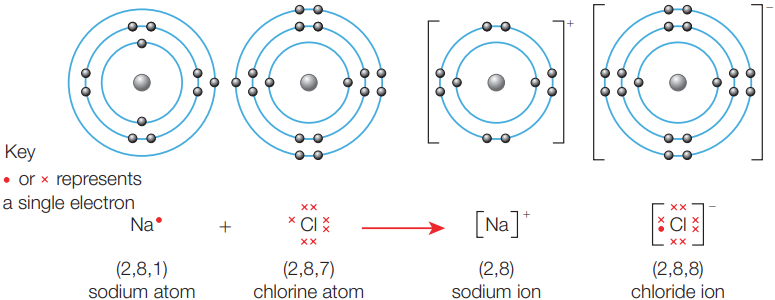
\includegraphics[scale=0.8]{Biology/1A/Images/1A-1-1.png}
        \caption{The formation of sodium chloride.}
    \end{figure}
\end{itemize}

\paragraph{Covalent Bonding}
